\documentclass[tikz,border=12pt]{standalone}
\usepackage[T1]{fontenc}
\usepackage{lmodern}
\usetikzlibrary{positioning,arrows.meta,fit,shapes.geometric}

\begin{document}
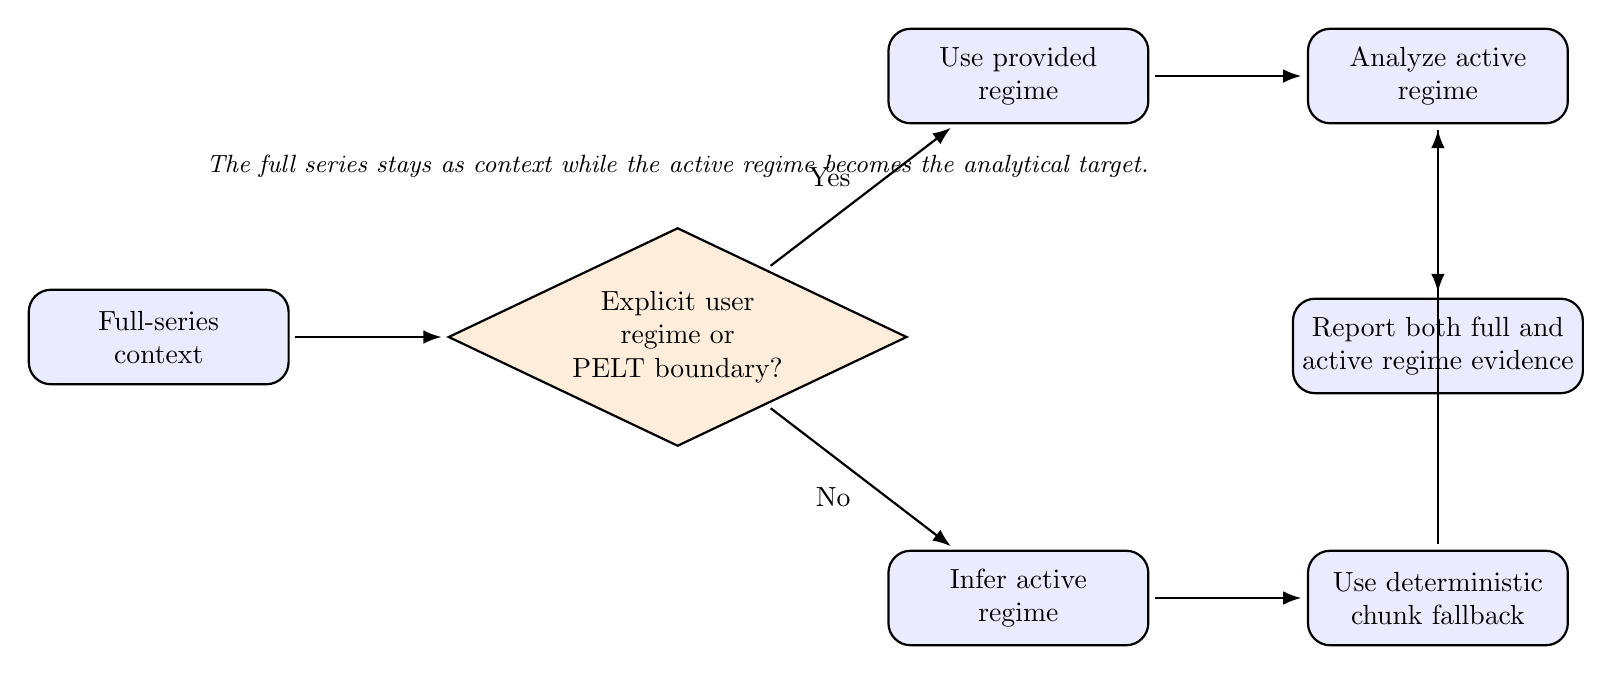
\begin{tikzpicture}[
  box/.style={draw, rounded corners=8pt, align=center, minimum width=3.3cm, minimum height=1.2cm, fill=blue!8, line width=0.8pt},
  decision/.style={draw, diamond, align=center, aspect=2.1, fill=orange!14, line width=0.8pt},
  note/.style={font=\small\itshape, align=center},
  arrow/.style={-Latex, thick, shorten >=2pt, shorten <=2pt}
]

\node[box] (full) {Full-series\\context};
\node[decision, right=2.0cm of full] (seg) {Explicit user\\regime or\\PELT boundary?};
\node[box, above right=2.0cm and 1.2cm of seg] (user) {Use provided\\regime};
\node[box, below right=2.0cm and 1.2cm of seg] (pelt) {Infer active\\regime};
\node[box, right=2.0cm of pelt] (fallback) {Use deterministic\\chunk fallback};
\node[box, right=2.0cm of user] (final) {Analyze active\\regime};
\node[box, below=2.2cm of final] (report) {Report both full and\\active regime evidence};

\draw[arrow] (full) -- (seg);
\draw[arrow] (seg) -- node[above left]{Yes} (user);
\draw[arrow] (seg) -- node[below left]{No} (pelt);
\draw[arrow] (pelt) -- (fallback);
\draw[arrow] (user) -- (final);
\draw[arrow] (fallback) -- (final);
\draw[arrow] (final) -- (report);

\node[note, above=0.5cm of seg] {The full series stays as context while the active regime becomes the analytical target.};

\end{tikzpicture}
\end{document}
